\documentclass[10pt]{beamer}
\usepackage[norsk]{babel}
\usepackage[utf8]{inputenc}

% Beamertheme
\usetheme{Szeged}
\usefonttheme{professionalfonts}
\usecolortheme{lily}

% Pakker
\usepackage{graphicx}
\usepackage{hyperref}
\usepackage{soul}
\usepackage{amsmath}
\usepackage{tikz}
\usepackage{listings}

% Tittel
\title{Introduksjon til \LaTeX{}}
\author{Veronika Heimsbakk\\veronika.heimsbakk@acando.no}
\date{}


\begin{document}

% Tittelramme
\begin{frame}\frametitle{}
\maketitle
\end{frame}

% Om meg
\begin{frame}\frametitle{Om meg}
\begin{description}
\item[Veronika Heimsbakk], utvikler i 
\includegraphics[width=1.4cm]{img/acandologo.png}
\end{description}

\begin{itemize}
	\item
	Utstudert fra Institutt for informatikk våren 2015.
	\item
	Forkjærlighet for \LaTeX{}, Ti\textit{k}Z, farger og fonter.
	\item
	Tidligere ansatt i Sonen $\heartsuit$.
	\item
	Favorittfag: INF2080 og INF2220.
\end{itemize}
\end{frame}

% Hva er LaTeX?
\section{Hva er \LaTeX{}?}
\subsection{}
\begin{frame}\frametitle{}

\begin{center}
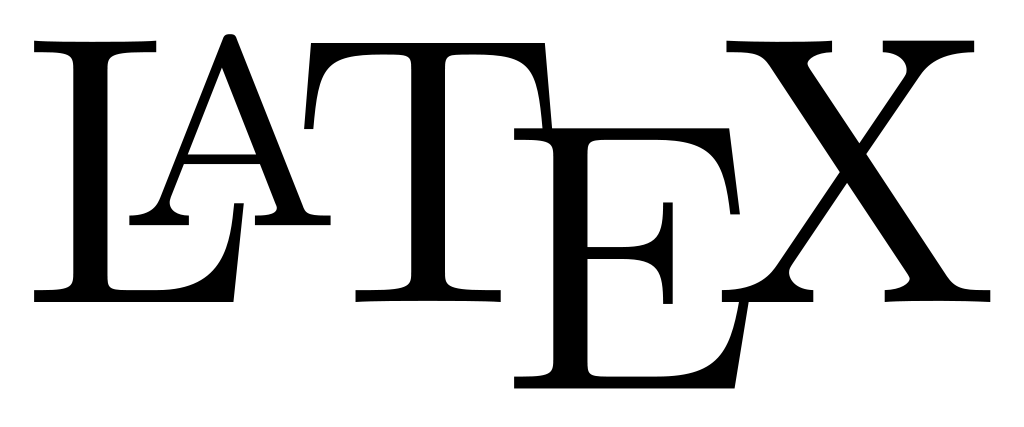
\includegraphics[width=5cm]{img/latexlogo.png}
\end{center}

\begin{itemize}
	\item
	Et dokument markup språk.
	\item
	Lansert i 1984.
	\item
	\LaTeX er en forkortelse for \textbf{Lamport} \textbf{\TeX}.
\end{itemize}
\end{frame}

% Lamport
\begin{frame}\frametitle{Leslie Lamport}

\begin{center}
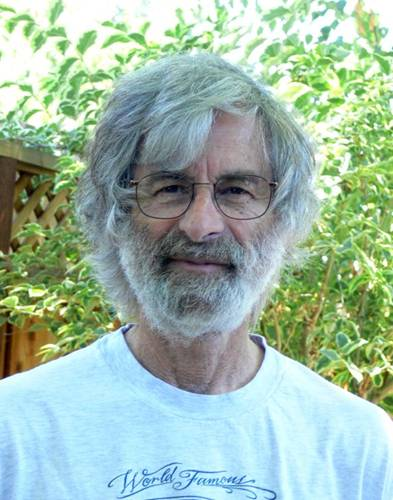
\includegraphics[height=3cm]{img/lamport.jpg}
\end{center}

\begin{itemize}
	\item
	Fikk ACM Turing Award i 2013 for sitt arbeid med distribuerte systemer.
\end{itemize}
\end{frame}

% TeX
\begin{frame}\frametitle{\TeX}

\begin{center}
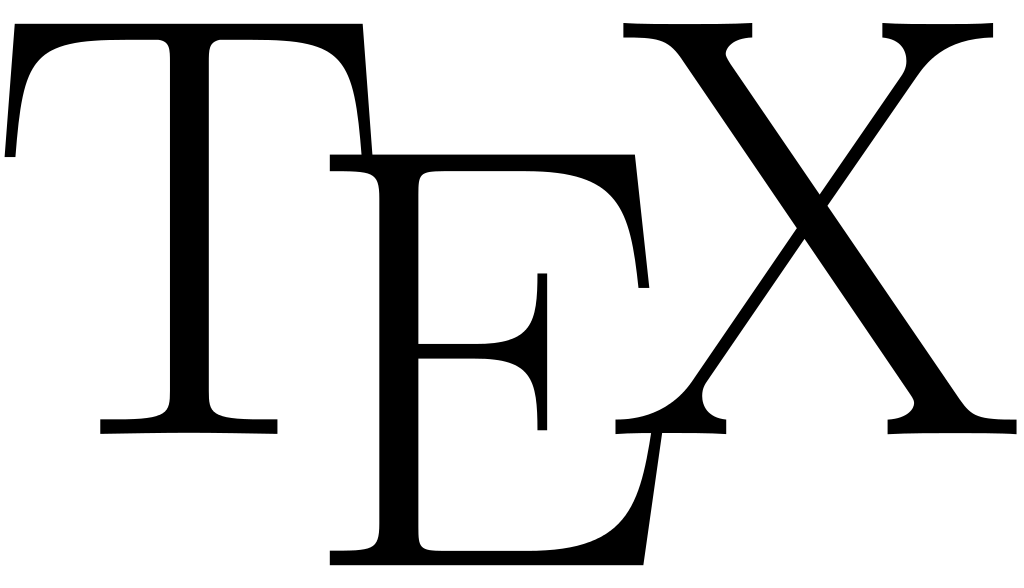
\includegraphics[width=3cm]{img/texlogo.png}
\end{center}

\begin{itemize}
	\item
	Lansert i 1978 av Donald Knuth.
	\item
	Typesetting system.
	\item
	Utviklet for at hvem som helst kunne lage bøker av høy kvalitet på hvilken som helst maskin.
	\item
	\url{https://www.tug.org/texlive/devsrc/Build/source/texk/web2c/tex.web}
\end{itemize}
\end{frame}

% Knuth
\begin{frame}\frametitle{Donald Knuth}

\begin{center}
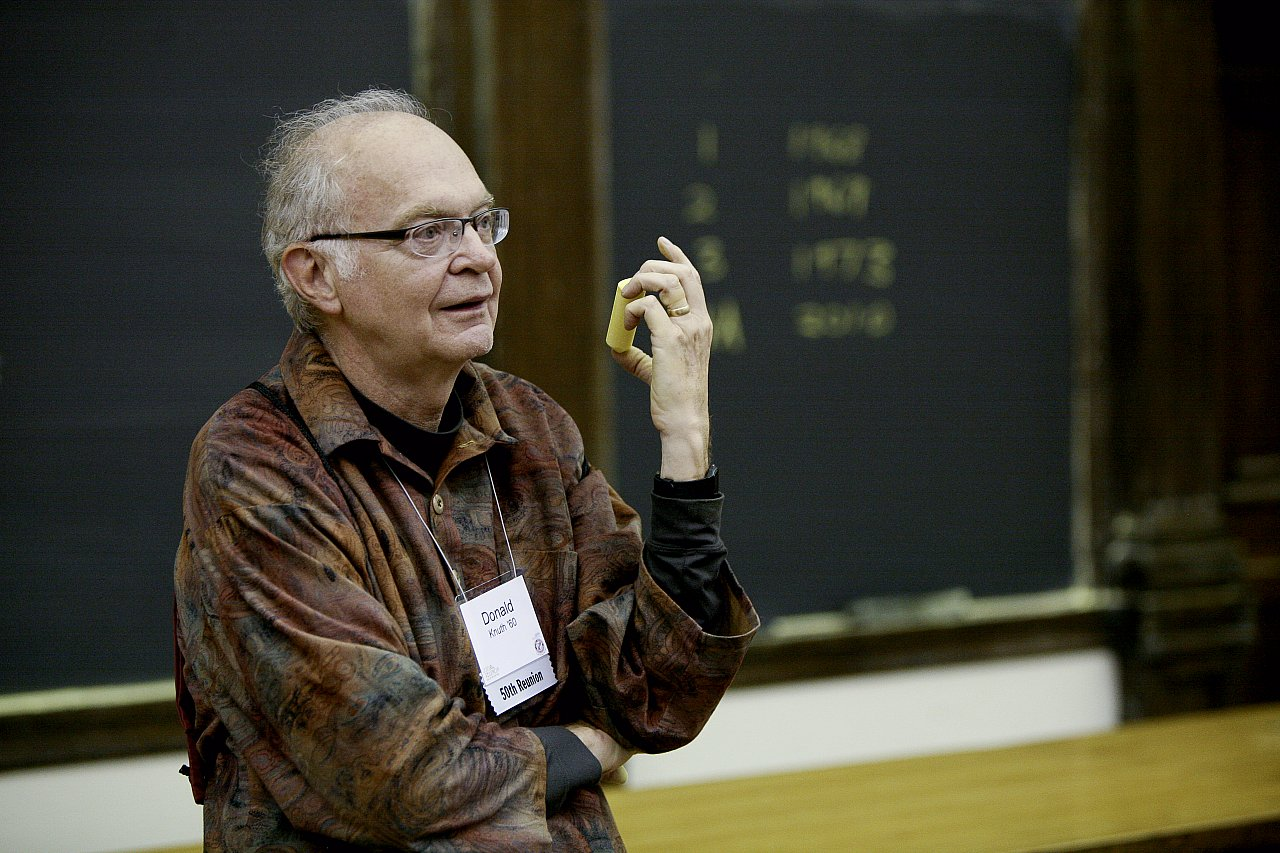
\includegraphics[height=3cm]{img/knuth.jpg}
\end{center}

\begin{itemize}
	\item
	The Art of Computer Programming
	\item
	«father of the analysis of algorithms»
\end{itemize}
\end{frame}

% Hvordan bruke LaTeX?
\section{Hvordan bruke \LaTeX{}?}
\subsection{}
\begin{frame}\frametitle{Innstallasjon}

\begin{center}

\includegraphics[width=1cm]{img/texworkslogo.png}
\end{center}

\begin{itemize}
	\item
	TeXworks, Kile, Vim, Emacs etc.
	\item
	\LaTeX er innstallert på alle Ifis maskiner.
	\item
	\texttt{apt-get install texlive}
\end{itemize}
\end{frame}

% Syntax
\section{Syntaks}
\subsection{}
\begin{frame}[fragile]\frametitle{Mitt første dokument}

\begin{verbatim}
\documentclass[a4paper, 10pt]{article}

\begin{document}
  Mitt første dokument!
\end{document}
\end{verbatim}

\begin{itemize}
	\item Det fins mange opsjoner for \texttt{documentclass}.
\end{itemize}

\begin{verbatim}
\documentclass[options]{class}
\end{verbatim}

\begin{itemize}
	\item \textbf{Options}: font size, paper size, twoside/oneside, landscape etc.
	\item \textbf{Class}: \texttt{book}, \texttt{article}, \texttt{report}, \texttt{minimal}, \texttt{beamer} etc.
\end{itemize}
\end{frame}

% Pakker
\begin{frame}[fragile]\frametitle{Pakker}

\begin{itemize}
	\item For oppsett av språk og fonter.
\end{itemize}

\begin{verbatim}
\usepackage[norsk]{babel} 
\usepackage[utf8]{inputenc} 
\usepackage[T1]{fontenc} 
\end{verbatim}

\begin{itemize}
	\item Det finnes \textit{mange} pakker for diverse snadder! Mer om dette litt senere.
\end{itemize}

\begin{verbatim}
\usepackage{hyperref}
\usepackage{mathtools}
\usepackage{listings}
\usepackage{graphicx}
\end{verbatim}
\end{frame}

% Forfatter og tittel
\begin{frame}[fragile]\frametitle{Forfatter og tittel}

\begin{verbatim}
\title{Introduksjon til \LaTeX}
\author{Veronika Heimsbakk\\veronika.heimsbakk@acando.no}

\begin{document}
  \maketitle
\end{document}
\end{verbatim}

\end{frame}

% Seksjoner
\begin{frame}[fragile]\frametitle{Seksjoner}

\begin{verbatim}
\section{Seksjon}
Dette er seksjon 1!

\subsection{Underseksjon}
Dette er seksjon 1 sin underseksjon.

\subsubsection{Underunderseksjon}
Dette er seksjon 1 sin underunderseksjon.
\end{verbatim}

\end{frame}

% Paragrafer
\begin{frame}[fragile]\frametitle{Paragrafer}

\begin{verbatim}
\paragraph{Paragraf}
Dette er en paragraf i seksjon 1 sin underunderseksjon.

\subparagraph{Underparagraf}
Dette er en underparagraf i seksjon 1 sin underunderseksjon.
\end{verbatim}

\end{frame}

% Kommentarer og ny linje
\begin{frame}[fragile]\frametitle{Kommentarer og ny linje}

\begin{verbatim}
% Dette er en kommentar.

\newline
\\
\end{verbatim}

\end{frame}

% Tekst
\section{Tekst}
\subsection{}
\begin{frame}[fragile]\frametitle{Tekst}

\begin{center}
\begin{tabular}{cccc}
\texttt{\textbackslash textbf}&\texttt{\textbackslash textit}&\texttt{\textbackslash texttt}&\texttt{\textbackslash underline}\\
\\
\textbf{Fet}&\textit{Kursiv}&\texttt{Typeface}&\underline{Understrek}\\
\end{tabular}
\end{center}

\begin{itemize}
	\item
	Flere måter å dekorere teksten på.
\end{itemize}

\begin{verbatim}
\textbf{Fet}
\bfseries{Fet}

\textit{Kursiv}
\itshape{Kursiv}
\end{verbatim}

\end{frame}

% Pakker
\begin{frame}[fragile]\frametitle{Tekst, pakker}

\begin{itemize}
	\item
	Fins flere pakker for tekstdekorering.
	\item
	\texttt{soul}, \texttt{color}, $\dots$
\end{itemize}

\begin{center}
\begin{tabular}{cc}
\texttt{\textbackslash st}&\texttt{\textbackslash textcolor\{red\}\{Rød tekst\}}\\
\\
\st{Gjennomstreking}&\textcolor{red}{Rød tekst}\\
\\
\texttt{\textbackslash caps}&\texttt{\textbackslash so}\\
\caps{Small Capitals}&\so{luftige bokstaver}
\end{tabular}
\end{center}

\end{frame}

% Størrelser
\begin{frame}[fragile]\frametitle{Tekst, størrelser}

\begin{tabular}{ll}
\texttt{\textbackslash tiny} & {\tiny Eksempeltekst}\\
\texttt{\textbackslash scriptsize}& {\scriptsize Eksempeltekst}\\
\texttt{\textbackslash footnotesize}& {\footnotesize Eksempeltekst}\\
\texttt{\textbackslash small}& {\small Eksempeltekst}\\
\texttt{\textbackslash normalsize}& {\normalsize Eksempeltekst}\\
\texttt{\textbackslash large}& {\large Eksempeltekst}\\
\texttt{\textbackslash Large}& {\Large Eksempeltekst}\\
\texttt{\textbackslash LARGE}& {\LARGE Eksempeltekst}\\
\texttt{\textbackslash huge}& {\huge Eksempeltekst}\\
\texttt{\textbackslash Huge}& {\Huge Eksempeltekst}
\end{tabular}

\end{frame}

% Skrifttyper
\begin{frame}[fragile]\frametitle{Tekst, skrifttyper}

\begin{tabular}{ll}
\texttt{\textbackslash normalfont} & {\normalfont Eksempeltekst}\\
\texttt{\textbackslash rmfamily}& {\rmfamily Eksempeltekst}\\
\texttt{\textbackslash sffamily}& {\sffamily Eksempeltekst}\\
\texttt{\textbackslash ttfamily}& {\ttfamily Eksempeltekst}\\
\end{tabular}

\begin{itemize}
	\item
	Det fint \textbf{mange} skrifttyper til \LaTeX{}. Sjekk ut \url{http://www.tug.dk/FontCatalogue/}
\end{itemize}

\end{frame}

% Verktøy
\section{Verktøy}
\subsection{}

% Tabeller
\begin{frame}[fragile]\frametitle{Tabeller}

\begin{verbatim}
\begin{tabular}[h!]{|l|r|c|}
  \textbf{Tabell}&\textbf{Tabell}&\textbf{Tabell}\\
  \hline
  en&to&tre\\
  fire&fem&seks\\
  sju&åtte&ni
\end{tabular}
\end{verbatim}

\end{frame}

% Figurer
\begin{frame}[fragile]\frametitle{Figurer}

\begin{verbatim}
\begin{figure}[h!]
  \centering
  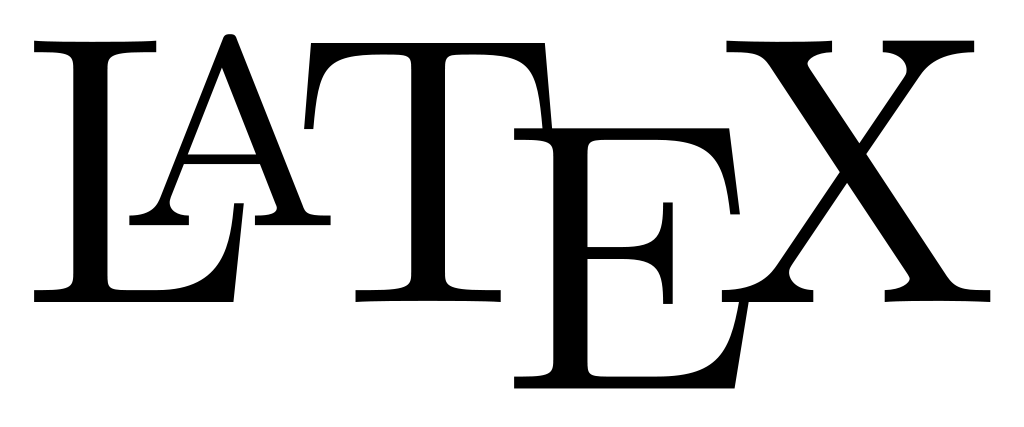
\includegraphics[width=\textwidth]{img/latexlogo.png}
  \caption{\LaTeX logo.}
\end{figure}
\end{verbatim}

\end{frame}

% Itemize
\begin{frame}[fragile]\frametitle{Lister, itemize}

\begin{itemize}
	\item
	Dette er et listelement.
	\item
	Dette er et listelement til.
\end{itemize}

\begin{verbatim}
\begin{itemize}
  \item
    Dette er et listelement.
  \item
    Dette er et listelement til.
\end{itemize}
\end{verbatim}

\end{frame}

% Enumerate
\begin{frame}[fragile]\frametitle{Lister, enumerate}

\begin{enumerate}
	\item
	Dette er et listelement.
	\begin{enumerate}
		\item
		Dette er et listelement til.
	\end{enumerate}
\end{enumerate}

\begin{verbatim}
\begin{enumerate}
  \item
    Dette er et listelement.
  \begin{enumerate}
    \item
      Dette er et listelement til.
  \end{enumerate}
\end{enumerate}
\end{verbatim}

\end{frame}

% Description
\begin{frame}[fragile]\frametitle{Lister, description}

\begin{description}
	\item[*] Dette er et listelement.
	\item[Element] Dette er et listelement til.
\end{description}

\begin{verbatim}
\begin{description}
  \item[*] Dette er et listelement.
  \item[Element] Dette er et listelement til.
\end{description}
\end{verbatim}

\end{frame}

% Emph, fotnoter, verbatim
\begin{frame}[fragile]\frametitle{Emph, fotnoter og verbatim}

\begin{itemize}
	\item
	I \texttt{verbatim} er \textit{alt} lov (bortsett fra \texttt{verbatim}).
\end{itemize}

\begin{verbatim}
Dette er en verbatim.
\end{verbatim}

\emph{Dette er en emph.}

Eksempeltekst med fotnote.\footnote{Dette er en fotnote.}

\begin{verbatim}
\emph{ ... }
\footnote{ ... }
\end{verbatim}

\end{frame}

% URLer
\begin{frame}[fragile]\frametitle{URLer}

\begin{itemize}
	\item
	Inkluderer pakken \texttt{hyperref}.
\end{itemize}

\begin{description}
	\item[]
	\url{http://tug.org/}
	\item[]
	\href{http://tug.org/}{\TeX{} Users Group web site}
	\item[]
	\href{mailto:veronahe@ifi.uio.no}{veronahe@ifi.uio.no}
\end{description}

\begin{verbatim}
\url{http://tug.org/}
\href{http://tug.org/}{\TeX{} Users Group web site}
\href{mailto:veronahe@ifi.uio.no}{veronahe@ifi.uio.no}
\end{verbatim}

\end{frame}

% Matematikk
\section{Matematikk}
\subsection{}
\begin{frame}[fragile]\frametitle{Miljø, fra \TeX{}}

\begin{verbatim}
$ ... $   % Formel på linje
$$ ... $$ % Fremhevet ligning
\end{verbatim}

Formel på linje $\forall x \in X, \quad \exists y \leq \epsilon$

Fremhevet ligning $$\forall x \in X, \quad \exists y \leq \epsilon$$ 

\end{frame}

\begin{frame}[fragile]\frametitle{Miljø, nytt i \LaTeX{}}

\begin{verbatim}
\( ... \)  % Formel på linje
\[ ... \]  % Fremhevet ligning
\end{verbatim}

Formel på linje \(\forall x \in X, \quad \exists y \leq \epsilon\)

Fremhevet ligning \[\forall x \in X, \quad \exists y \leq \epsilon\]

\begin{itemize}
	\item
	Alternative måter å skrive ligninger på er ved å bruke
	\begin{itemize}
		\item
		\texttt{\textbackslash begin\{equation\}}
		\item
		\texttt{\textbackslash begin\{align\}}
	\end{itemize}
\end{itemize}

\begin{align}
\forall x \in X, \quad \exists y \leq \epsilon
\end{align}

\begin{itemize}
	\item
	\texttt{align} gir nummererte ligninger.
\end{itemize}
\end{frame}

% Symboler
\begin{frame}[fragile]\frametitle{Symboler}

\begin{center}
\begin{tabular}{ll}
Symbol&Skript\\
\hline
$\cap$&\texttt{\textbackslash cap}\\
$\cup$&\texttt{\textbackslash cup}\\
$\subseteq$&\texttt{\textbackslash subseteq}\\
$\equiv$&\texttt{\textbackslash equiv}\\
$\in$&\texttt{\textbackslash in}\\
$\notin$&\texttt{\textbackslash notin}\\
$\land$&\texttt{\textbackslash land}\\
$\lor$&\texttt{\textbackslash lor}\\
$\models$&\texttt{\textbackslash models}\\
$\emptyset$&\texttt{\textbackslash emptyset}\\
$\Lambda$&\texttt{\textbackslash Lambda}\\
$\lambda$&\texttt{\textbackslash lambda}\\
\end{tabular}
\end{center}

\begin{itemize}
	\item
	\href{http://texdoc.net/texmf-dist/doc/latex/comprehensive/symbols-a4.pdf}{The Comprehensive \LaTeX{} Symbol List}
	\item
	\href{https://en.wikibooks.org/wiki/LaTeX/Mathematics}{\LaTeX{} Wiki Mathematics}
\end{itemize}

\end{frame}

% Sannhetstabeller
\begin{frame}[fragile]\frametitle{Sannhetstabeller}

\LaTeX er det \textbf{perfekte} verktøy for dere som tar INF2080\footnote{Samt andre fag med tekstlige innleveringer.}!

\begin{center}
\begin{tabular}{cc|c}
A&B&A $\land$ B\\
\hline
0&0&0\\
0&1&0\\
1&0&0\\
1&1&1\\
\end{tabular}
\end{center}

\end{frame}

% Kode
\section{Kode}
\subsection{}

% Innstillinger for lstlistings
\lstset{
	language=Java,
	keywordstyle=\color{blue},
	stringstyle=\color{red},
	numbers=left,
	numberstyle=\tiny\color{lightgray},
	tabsize=2
}

\begin{frame}[fragile]
\frametitle{\texttt{lstlistings}}

\begin{lstlisting}
public class Kode {
	public static void main(String[] args) {
		System.out.println("Hei, alle sammen!");
	}
}
\end{lstlisting}
\end{frame}

\begin{frame}[fragile]
\frametitle{Innstillinger for \texttt{lstlistings}}
\begin{verbatim}
\lstset{
  language=Java,
  keywordstyle=\color{blue},
  stringstyle=\color{red},
  numbers=left,
  numberstyle=\tiny\color{lightgray},
  tabsize=2
}
\end{verbatim}
\end{frame}

\begin{frame}[fragile]
\frametitle{Bruke \texttt{lstlistings}}
\begin{verbatim}
\begin{lstlisting}
  public class Kode {
    public static void main(String[] args) {
      System.out.println("Hei, alle sammen!");
    }
  }
\end{lstlisting}
\end{verbatim}
\begin{itemize}
\item
Kan laste inn fil ved å bruke \texttt{\textbackslash lstinputlisting\{source\_filename.py\}}
\end{itemize}
\end{frame}

\begin{frame}
\frametitle{Språk som støttes av \texttt{lstlistings}}
ABAP, ACSL, Ada, Algol, Ant, Assembler, Awk, bash, Basic, C\#, C++, C, Caml, Clean, Cobol, Comal, csh, Delphi, Eiffel, Elan, erlang, Euphoria, Fortran, GCL, Gnuplot, Haskell, HTML, IDL, inform, Java, JVMIS, ksh, Lisp, Logo, Lua, make, Mathemathica, Matlab, Mercury, MetaPost, Miranda, Mizar, ML, Modelica, Modula-2, MuPAD, NASTRAN, Oberon-2, Objective C, OCL, Octave, Oz, Pascal, Perl, PHP, PL/I, Plasm, POV, Prolog, Promela, Python, R, Reduce, Rexx, RSL, Ruby, S, SAS, Scilab, sh, SHELXL, Simula, SQL, tcl, \TeX, VBScript, Verilog, VHDL, VRML, XML, XSLT.

\begin{itemize}
\item
Du kan også legge inn flere nøkkelord ved å bruke innstillingen \texttt{morekeywords} i \texttt{lstset}.
\end{itemize}
\end{frame}


% Veien videre
\section{Veien videre}
\subsection{}

% Mer informajson
\begin{frame}[fragile]\frametitle{Mer informasjon}
\begin{itemize}
\item
\url{http://www.mn.uio.no/ifi/tjenester/it/hjelp/latex/}
\item
\url{https://en.wikibooks.org/wiki/LaTeX}
\item
\url{http://tug.org/}
\end{itemize}

\end{frame}

% Takk for meg
\begin{frame}[fragile]\frametitle{Takk for meg!}
Ikke nøl med å ta kontakt på veronika.heimsbakk@acando.no!
\vspace{20pt}

{\Large \textbf{Neste foredrag}: Ti\textit{k}Z $\heartsuit$}

\vspace{20pt}

\def\firstcircle{(0,0) circle (1.5cm)}
\def\secondcircle{(45:2cm) circle (1.5cm)}
\def\thirdcircle{(0:2cm) circle (1.5cm)}

\scalebox{0.15}{
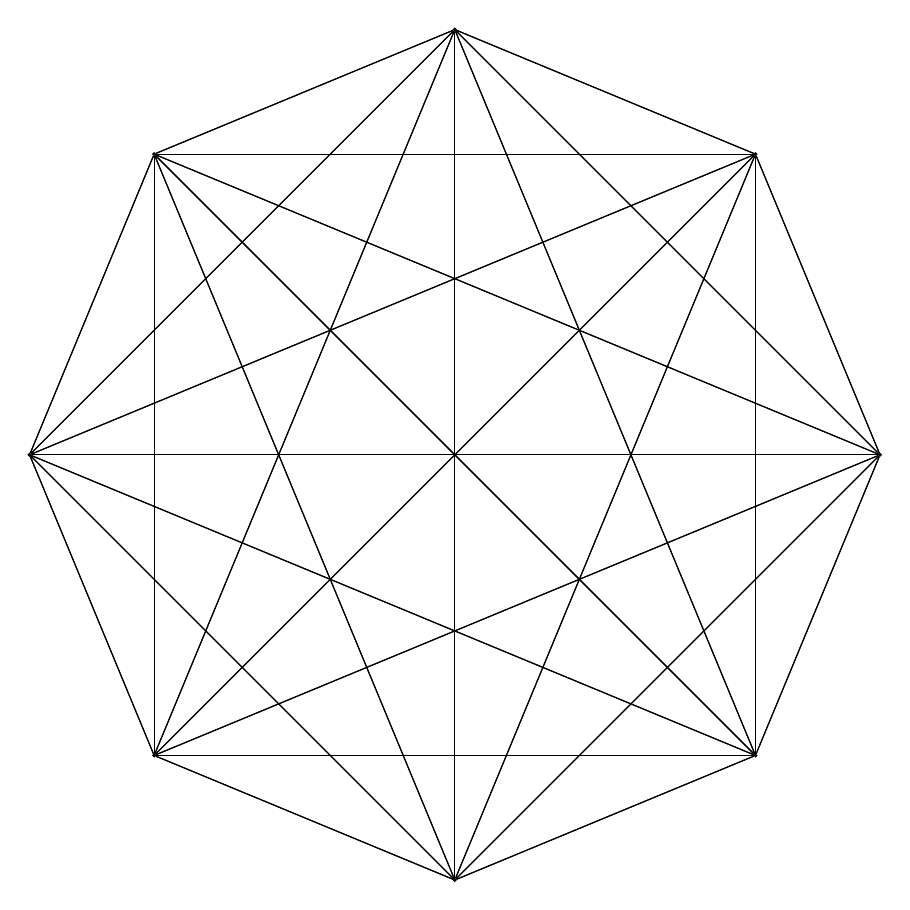
\begin{tikzpicture}
\foreach \x in {1,...,8}{%
	\pgfmathparse{(\x-1)*360/8}
	\node[draw,circle,inner sep=0.25, fill=purple] (N-\x) at (\pgfmathresult:5.4) {};
}
\foreach \x in {1,...,8}{%
	\foreach \y in {1,...,8}{%
		\path (N-\x) edge[black,-] (N-\y);
	}
}
\end{tikzpicture}
}
\scalebox{0.5}{
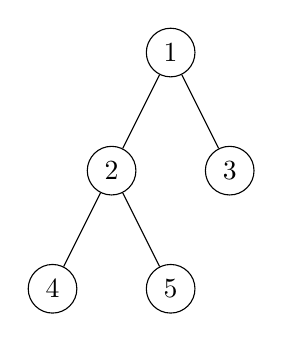
\begin{tikzpicture}[every node/.style={circle, draw=black}]
\node {1}
	child { node {2} 
		child { node {4} }
		child { node {5} }
	}
	child { node {3} }
;
\end{tikzpicture}
}
\scalebox{0.3}{
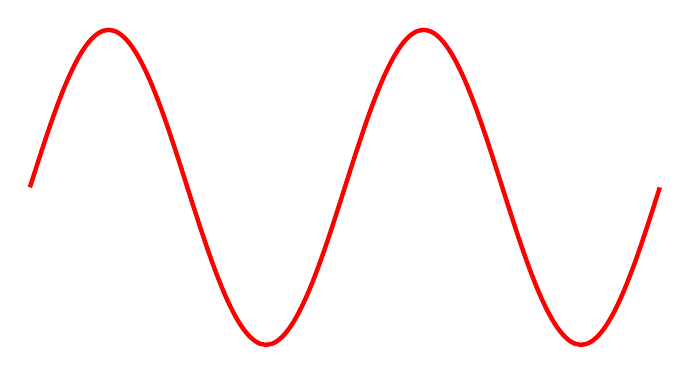
\begin{tikzpicture}
\draw[red, ultra thick] (0,0) sin (1,2) cos (2,0) sin (3,-2) cos (4,0) sin (5,2) cos (6,0) sin (7,-2) cos (8,0);
\end{tikzpicture}
}
\scalebox{0.8}{
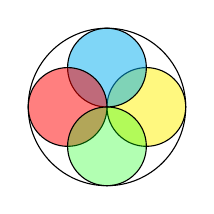
\begin{tikzpicture}
	\draw(6,0) circle (1cm);
	\draw[fill=yellow, fill opacity=0.5](6.5,0) circle (0.5);
	\draw[fill=cyan, fill opacity=0.5] (6,0.5) circle (0.5);
	\draw[fill=red, fill opacity=0.5](5.5,0) circle (0.5);
	\draw[fill=green, fill opacity=0.3](6,-0.5) circle (0.5);
\end{tikzpicture}
} 
\scalebox{0.4}{
\begin{tikzpicture}
        \begin{scope}[even odd rule]
            \clip \secondcircle (-0,-0) rectangle (0,0);
        \fill[teal] \firstcircle;
        \end{scope}
        \draw \firstcircle node {$A$};
        \draw \secondcircle node {$B$};
\end{tikzpicture}
}

\end{frame}

\end{document}